\documentclass[a4paper,12pt]{article}
\usepackage[latin1]{inputenc} %entrada usando ISO-Latin1
\usepackage{listings}
\usepackage{color}
\usepackage{a4wide}
\usepackage{graphicx}
\usepackage{subfig}
\usepackage{wrapfig}
\usepackage{hyperref}
\usepackage{listings}
\usepackage{amsmath} 
\lstset{
   breaklines=true,
   basicstyle=\ttfamily}
% \usepackage{draftwatermark}\usepackage[figurewithin=section,tablewithin=section]{caption}
%\usepackage{subfigure}

\pagestyle{headings}

\title{Accelerator simulations: Physics}
\author{LBNL LLRF Team}

\date{\today}

\begin{document}
\numberwithin{equation}{section} 
\maketitle
\setcounter{tocdepth}{3}
\tableofcontents

\newpage

\section{Introduction}

\begin{figure}
\centering
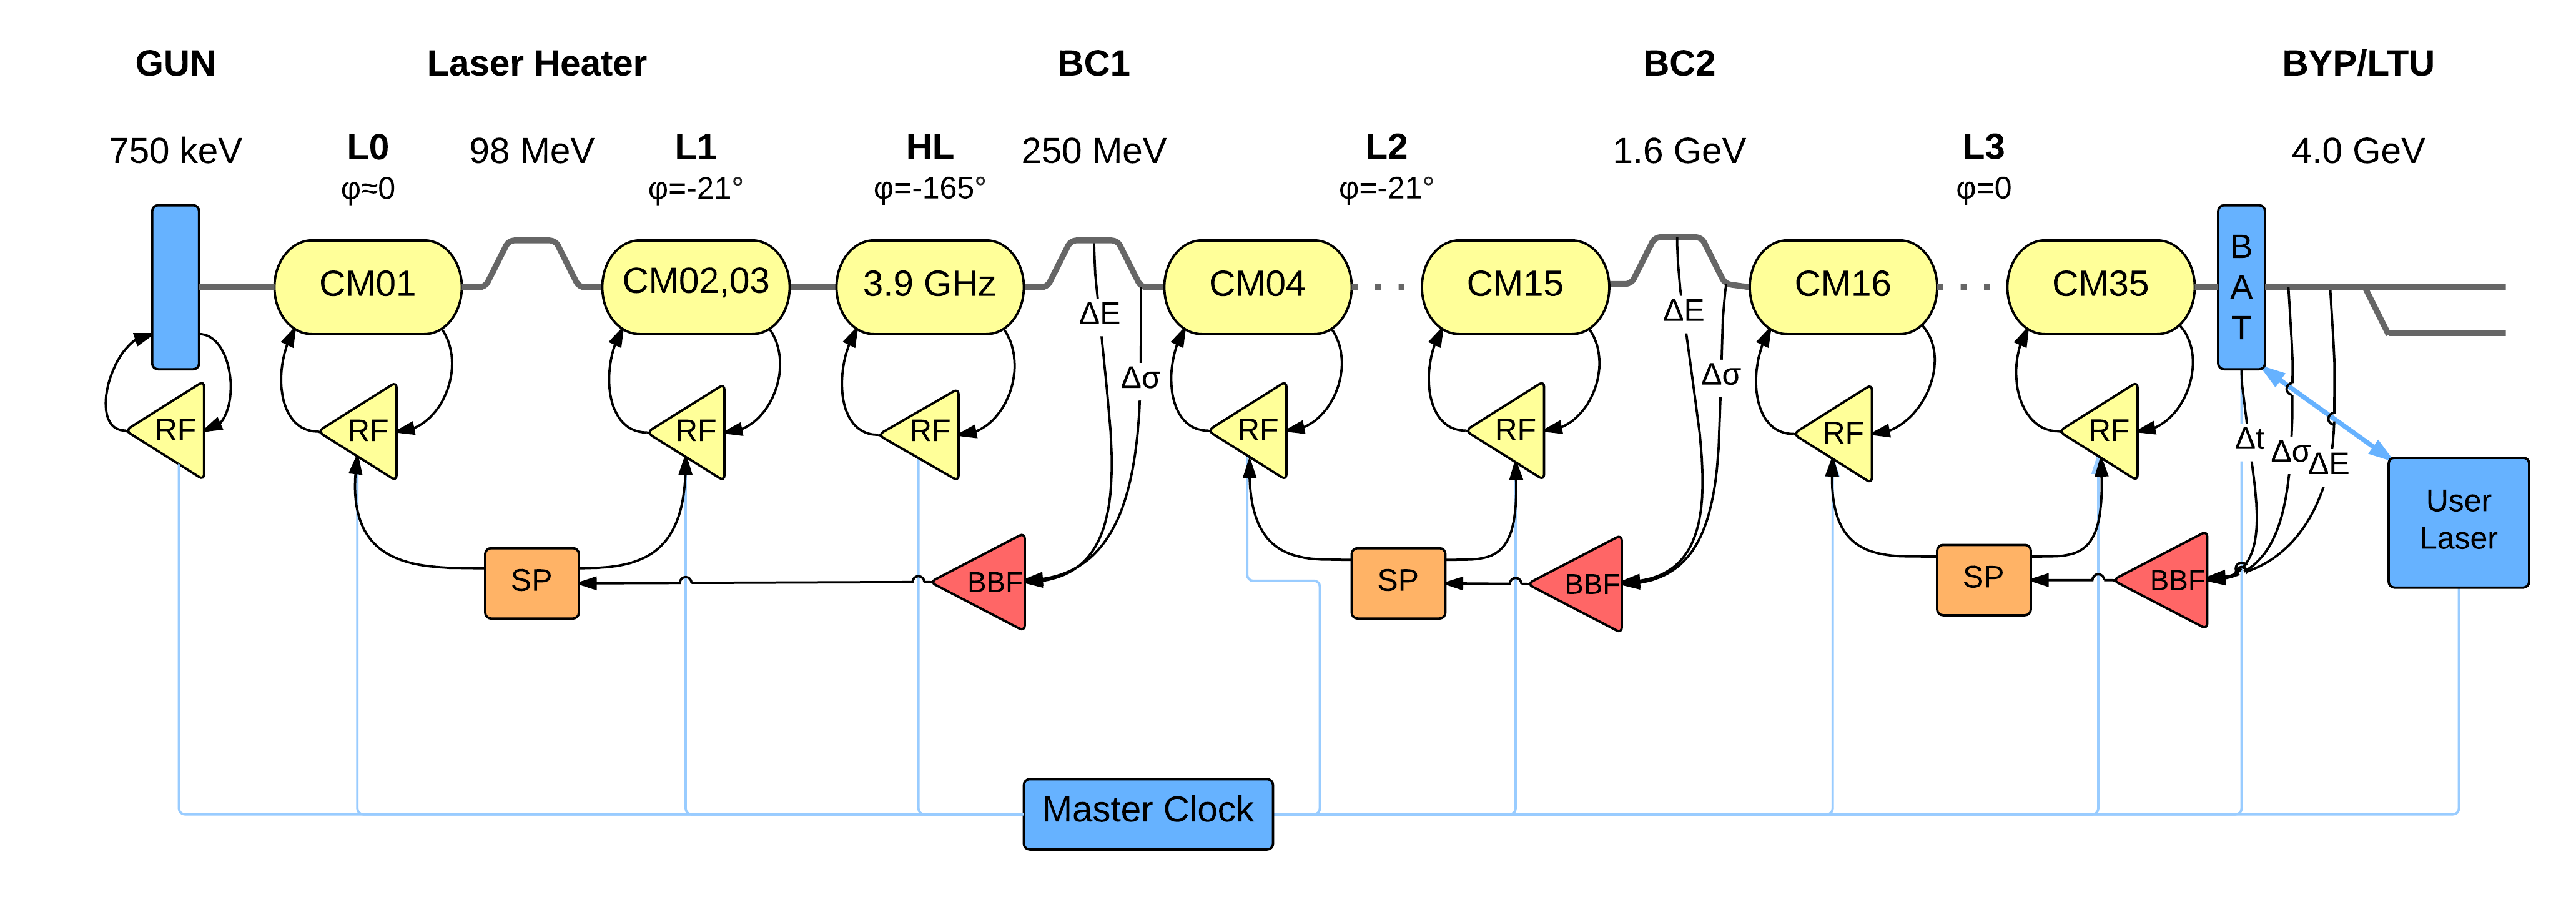
\includegraphics[scale=0.11]{../figures/LCLS-II_feedback_layout.png}
\caption{LCLS-II feedback layout.}
\label{fig:lclsII-feedback_layout}
\end{figure}

During the design, comissioning and operations of a Linac-driven FEL it is useful to have modeling capabilities to abstract and analyze some of the complex problems involved in LLRF and beam-based feedback in the confortable environment of computer simulations. The simulation framework presented here is a dramatic improvement of a previous version written in Octave/Matlab~\cite{ref:model-paper}, where extensively tested LLRF models are integrated with a longitudinal phase space tracking simulator~\cite{ref:litrack} along with the interaction between the two via beam-based feedback using a computionally efficient simulation engine. 

The models include beam instrumentation, considerations on loop delays for in both the LLRF and beam-based feedback loops, as well as the ability to inject noise (both correlated and uncorrelated) at different points of the machine including a full characterization of the electron gun performance parameters. The Linac is divided into generic compounds composed of an accerating section followed by a bunch compressor (where the bunch compressor can be enabled/disabled) and beam performance parameters are measured at any stage of the machine for characterization and/or for use to apply beam-based feedback. Time-series data is computed at a configurable repetition rate and results can be visualized in both time and frequency domain, including transfer functions between any noise source and beam performace parameters.


Figure~\ref{fig:lclsII-feedback_layout} shows a high-level representation of the LCLS-II layout, as configured at the time of this writing. The model described here represents each component of the machine in a way that configuration parameters can be adapted as the machine layout and configuration evolves (during the design or in future upgrades), where the contribution of each noise source (correlated or uncorrelated) to the machine performance budget can be quantified, including the ability to represent the effectiveness of different feedback loops to reduce noise contributions under different configurations. 

\section{Model hierarchy}

The accelerator model is intended to be modular in order to adapt to different configurations. The motivation behind this partitioning is to allow for different types of studies. For example, one can focus on some localized effects at the RF station level where only one station is simulated, or inspect how different cavities interact mechanically inside a cryomodule, or run studies at a machine level in order to analize slow beam-based feedback performance where not much detail on the internals of RF stations is desired.

\begin{figure}
\centering
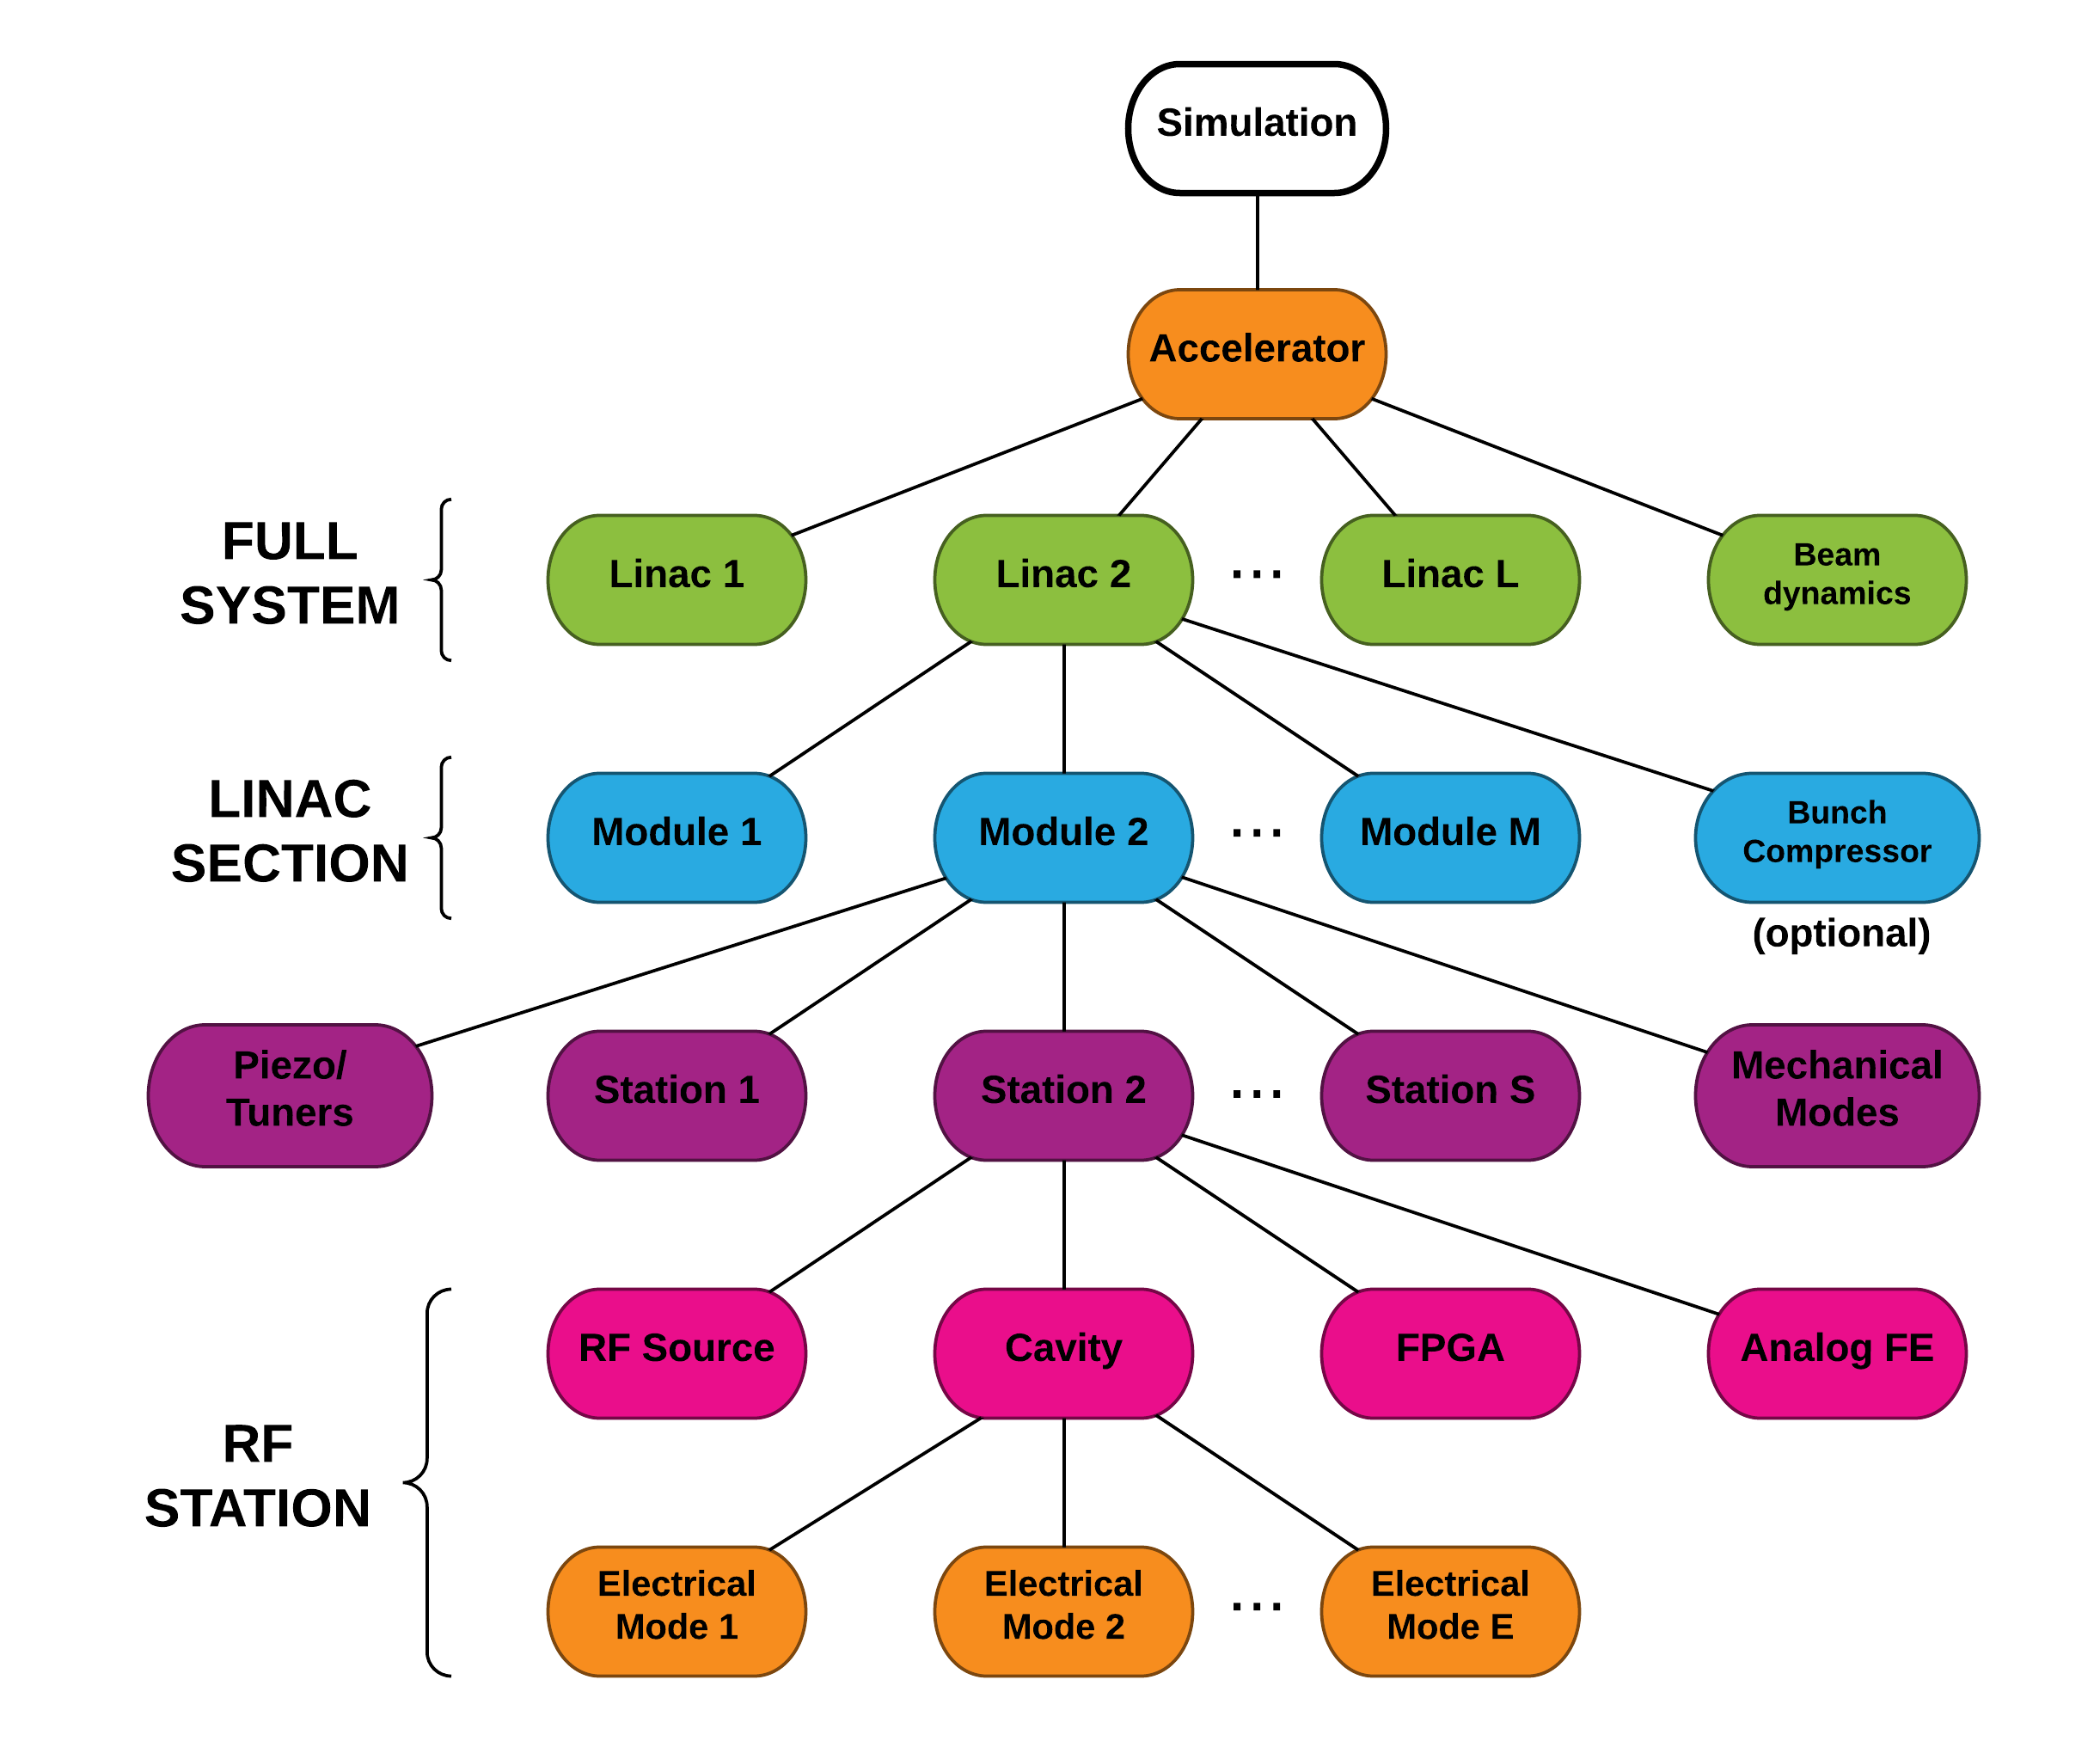
\includegraphics[scale=0.2]{../figures/Model_hierarchy.png}
\caption{Model hierarchy.}
\label{fig:model_hierarchy}
\end{figure}

The different model configurations described above are put in practice using a model hierarchy shown in Figure~\ref{fig:model_hierarchy}. The first component is a simulation entity, which describes simulation parameters such as time step size, total simulation time, etc. The simulation then includes an accelerator which can be composed of one or more Linac sections, including a longitudinal beam dynamics simulation to represent beam propagating from one Linac section to the next. One linac section is then represented as a series of cryomodules (or modules), optinally followed by a bunch compressor. This is the fundamental building block of the accelerator, where one can imagine to have the case of L1 in Fig.~\ref{fig:lclsII-feedback_layout} with two cryomodules and no bunch compressor, followed by HL (with different frequency, beam phase relative to the RF, etc), this time followed by a bunch compressor (BC1 in this case).

Each module is then represented by a collection of RF stations, including inter-station interactions through a model of the mechanical resonances in the cryomodule. The electro-mechanical couplings between the mechanical modes and individual electrical modes in the cavities are represented, as well as the effect of tuners and piezos on these resonances. Each station is composed of the typical RF system layout, with an N-cell cavity (including several normal modes), a high-power RF source, an FPGA controller, and the analog front-end (which represents anti-alias filtering, LLRF noise. etc). The last stage of the hierarchy is the cavity electrical modes, which each have their own resonance frequency, Q and couplings with mechanical modes in a module.

\begin{figure}
\centering
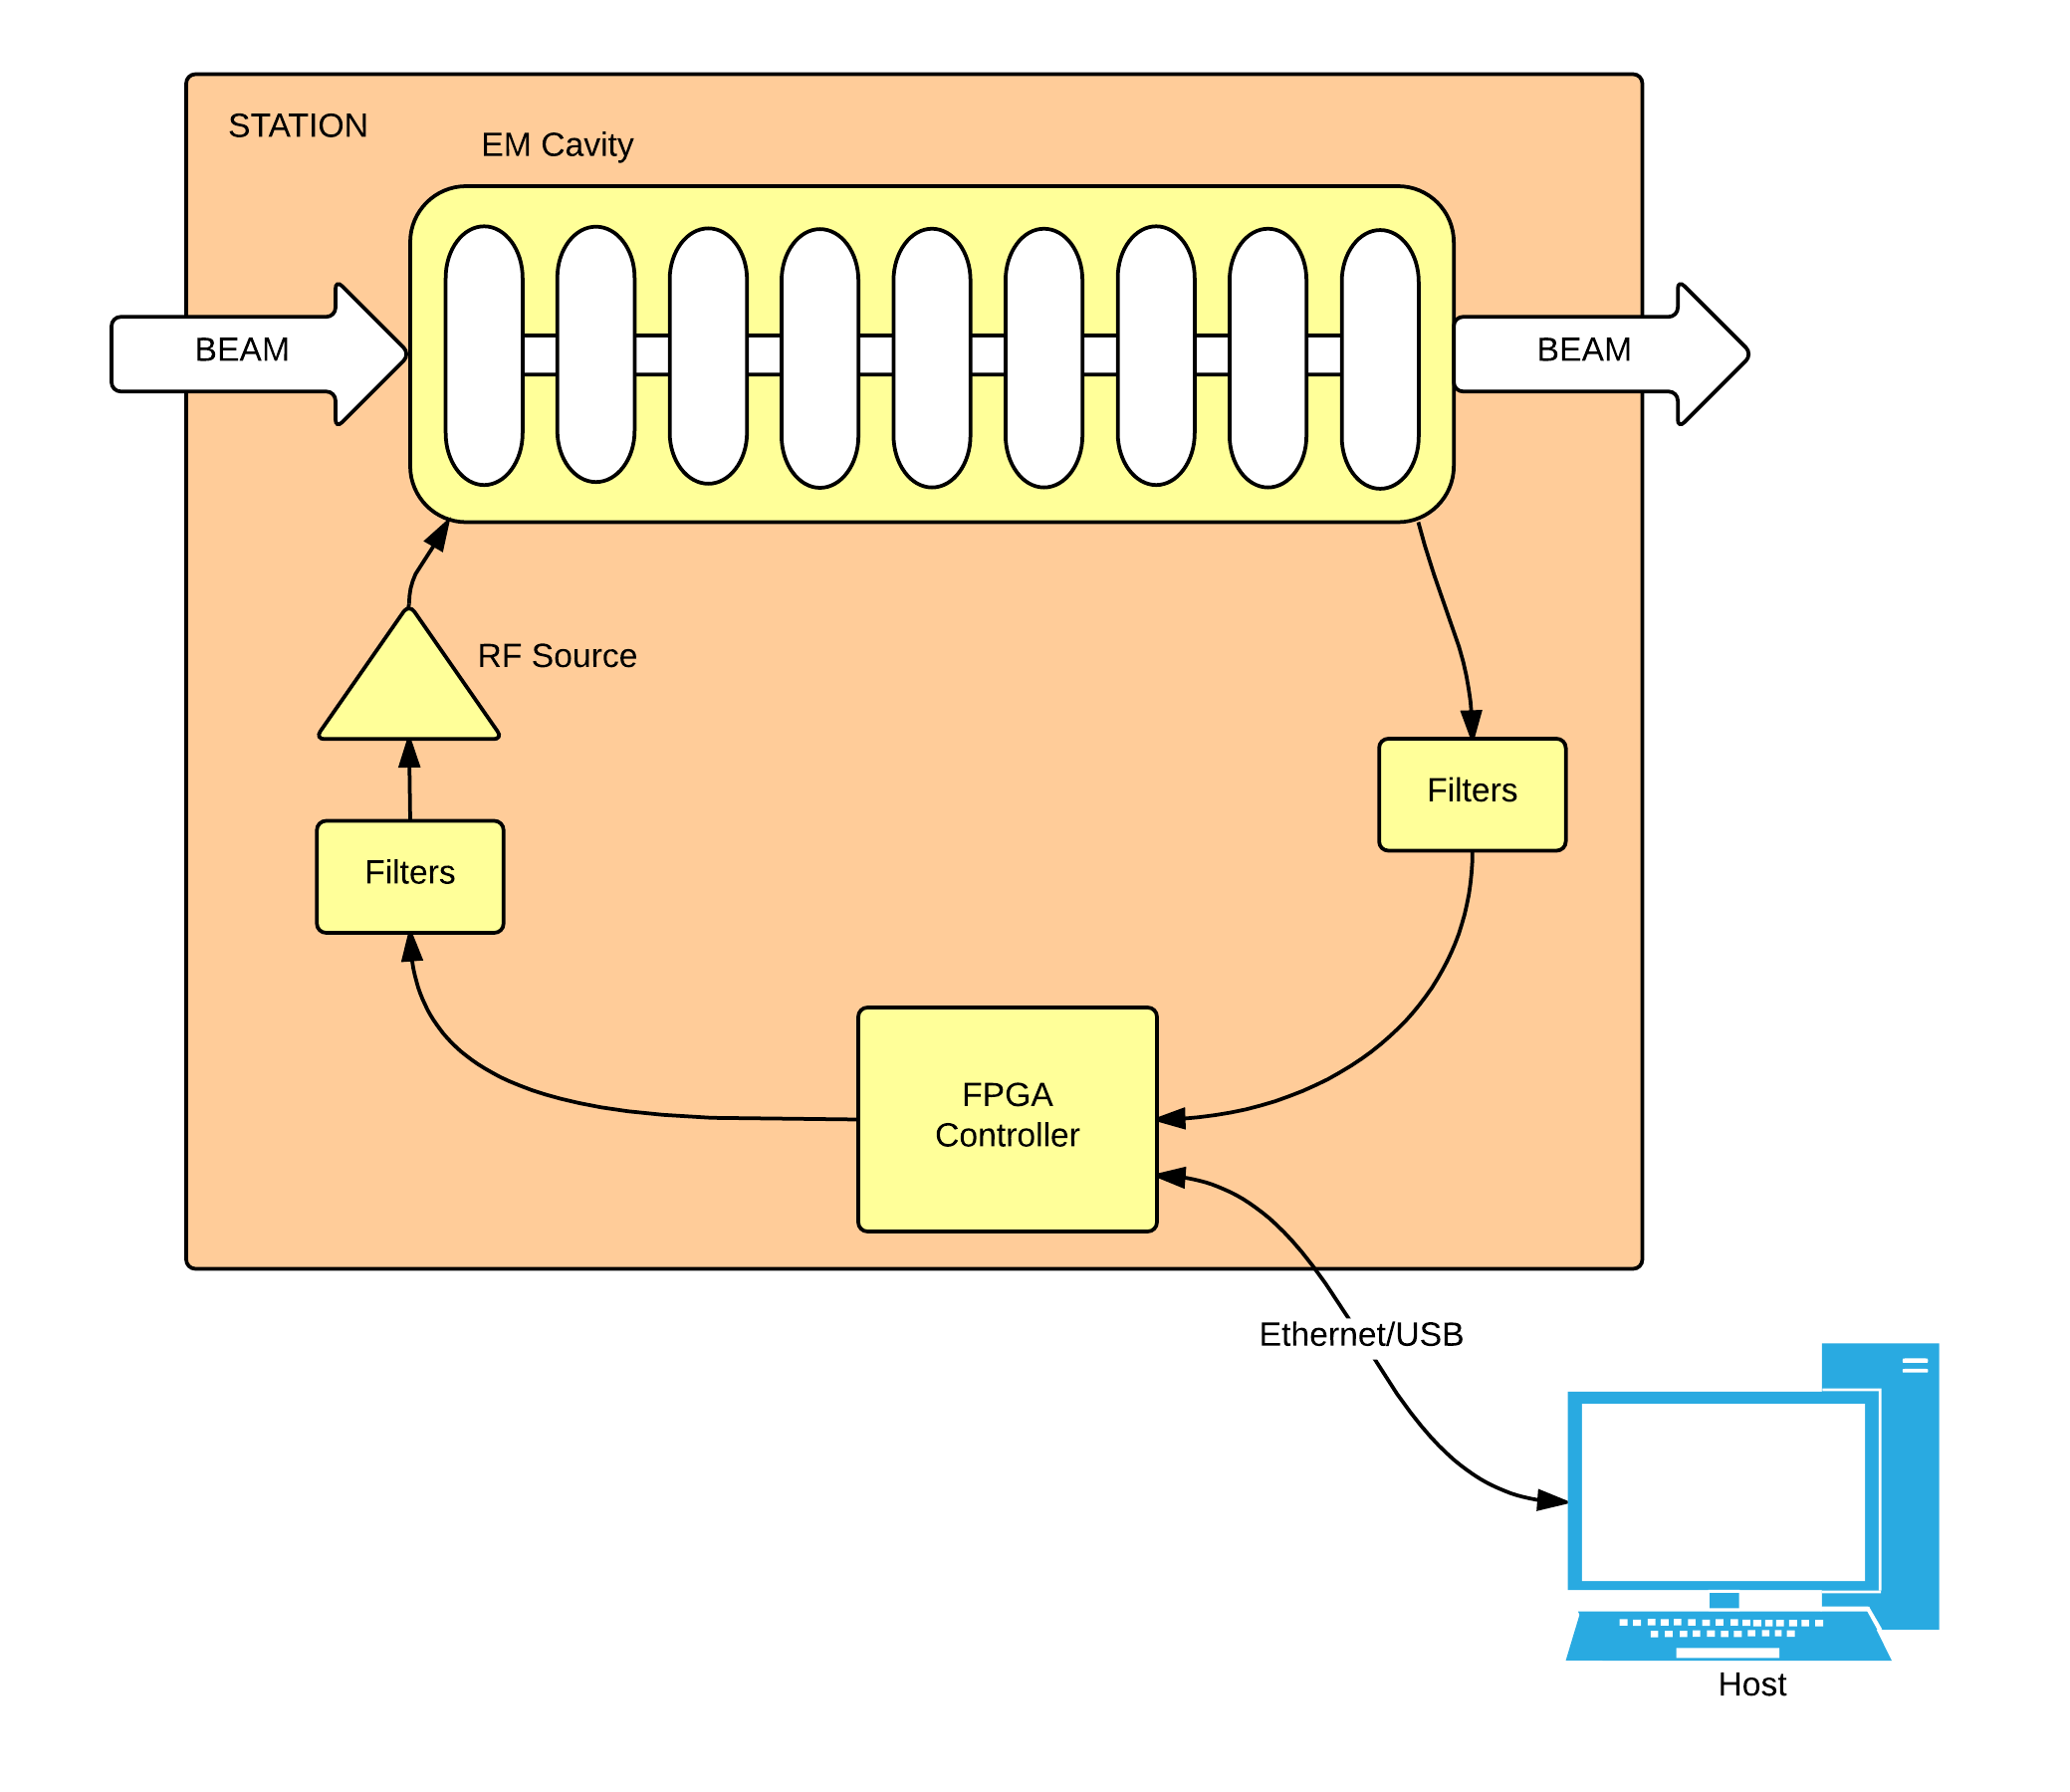
\includegraphics[scale=0.18]{../figures/Station_block_diagram.png}
\caption{Station block diagram.}
\label{fig:Station_block_diagram}
\end{figure}

In the next few sections we describe the models used in each layer of the hierarchy shown in Fig.~\ref{fig:model_hierarchy}, starting bottom up so that the reader progressively understands every component in each layer without making any assumptions.

\section{RF Station}

The RF station model responds to the typical RF system topology, with an FPGA-based system controlling the EM field inside an accelerating cavity as shown in Fig.~\ref{fig:Station_block_diagram}.
The model includes a multi-cell cavity (inlcuding different normal modes, detuning and its different couplings), an FPGA controller, a saturation model for the RF source, filters, etc.

The RF station is modeled at baseband, where up and down conversions in the real system are not considered and only the slowly varying amplitude and phase modulations (or In-phase and Quadrature, I\&Q) of a carrier at the RF reference frequency are represented. The FPGA controller in a real system typically works on I-Q sampled cavity fields. Representing the rest of the components in the RF station model at baseband allows for a more computationally efficient implementation of the simlation code, while not losing information of interest on the different signals. 

The different components of the RF station model are described in the rest of this section.

\subsection{Cavity model}


The cavity model described here responds to the typical multi-cell cavity structure, with couplings to the RF source, a probe, and the beam of particles. There are two aspects to representing this problem: the complete electro-magnetic field description inside the cavity and the equivalent circuit representation, where the field description is needed in order to define the equivalent-circuit using simulation codes like Superfish~\cite{ref:superfish}. It is convinient to use the equivalent-circuit representation in order to model the cavity behavior as well as its interactions with the RF system and the beam.

An RF cavity can be represented by a series of coupled resonators (one per cell in the cavity, each respresented by an RLC circuit~\cite{ref:montgomery}, as shown in Fig.~\ref{fig:cav_eq_circuit}). If we apply Kirchhoff's current law to the mode's RLC equivalent circuit, we get:

\begin{equation}
  \centering \vec I_{\rm cav} = \vec I_{\rm C} + \vec I_{\rm R} + \vec I_{\rm L}
  \label{eq:currents}
\end{equation}

where:

\begin{equation}
  \frac{d\vec I_{\rm C}}{dt} = C \cdot \frac{d^2\vec V}{dt^2}\text{,}\qquad \frac{d\vec I_{\rm R}}{dt} = \frac{1}{R_{\rm L}}\frac{d\vec V}{dt} \qquad \text{and}\qquad \frac{d\vec I_{\rm L}}{dt} = \vec V/L
  \label{eq:currents2}
\end{equation}

\begin{figure}
\centering
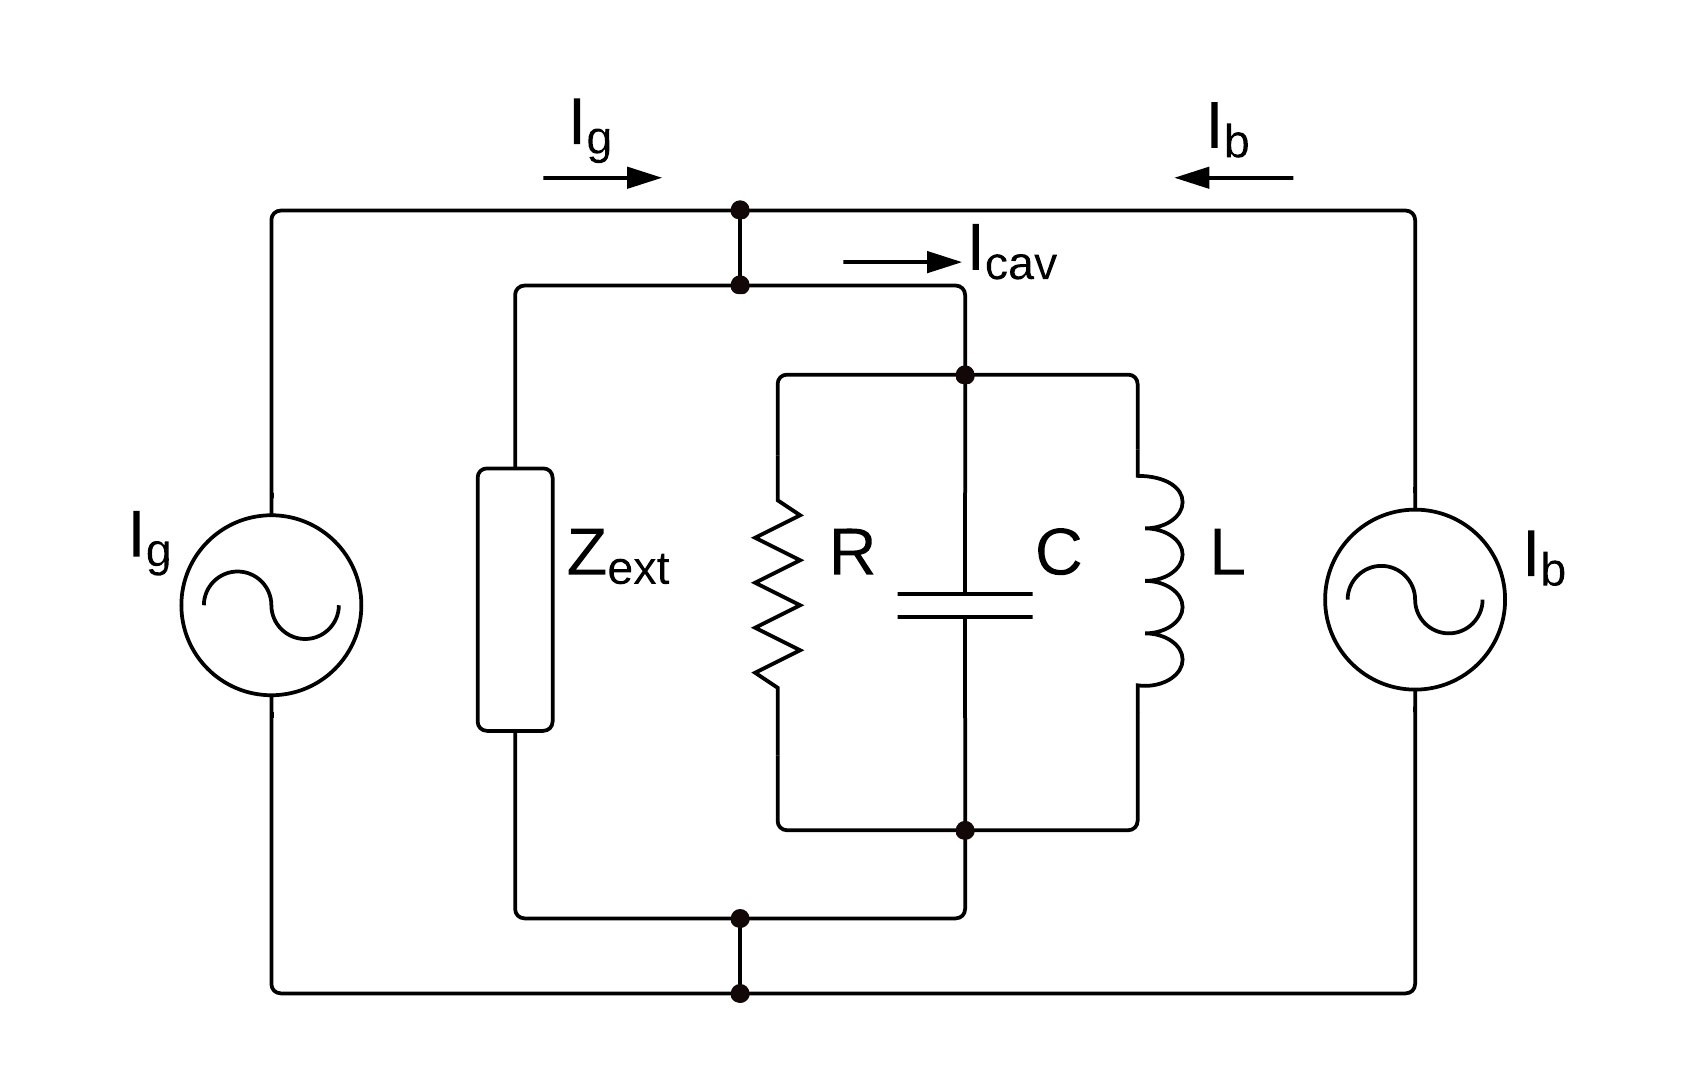
\includegraphics[scale=0.25]{../figures/cavity_eq_circuit.png}
\caption{Cavity equivalent circuit.}
\label{fig:cav_eq_circuit}
\end{figure}

Differentiating both sides of equation~\ref{eq:currents} and substituting using eq.~\ref{eq:currents2}, the full vector (complex) differential equation for the cavity accelerating voltage $\vec V$ can be written as:

\begin{equation}
  \frac{d^2\vec V}{dt^2} + \frac{1}{R_{\rm L}C}\frac{d\vec V}{dt} + \frac{1}{LC}\vec V = \frac{1}{C}\frac{d\vec I_{\rm cav}}{dt}
\end{equation}

which can be expressed as a function of the mode's nominal resonance frequency $\omega_0$ ($1/LC=\omega_0^2$) and loaded Q ($1/R_{\rm L}C=\omega_0/Q_{\rm L}$):
 
\begin{equation}
  \frac{d^2\vec V}{dt^2} + \frac{\omega_0}{Q_{\rm L}}\frac{d\vec V}{dt} + \omega_0^2 \vec V = \frac{\omega_0^2 R_{\rm L}}{Q_{\rm L}}\frac{d\vec I_{\rm cav}}{dt}
  \label{eq:2nd_order}
\end{equation}

Taking the slowly varying envelope approximation~\cite{ref:svea} and separating voltage and current into real and imaginary parts we can reduce the order of equation~\ref{eq:2nd_order} (a second-order band-pass filtered centered at the resonance frequency) to a first-order low-pass filter at baseband~\cite{ref:schilcher}:

\begin{equation}
  (1-j\frac{\omega_d}{\omega_f})\vec V + \frac{1}{\omega_f}\frac{d\vec V}{dt} = R_{\rm L} \vec I_{\rm cav}
  \label{eq:1st_order1}
\end{equation}

where $\omega_f=\omega_0/2Q_L$ is the mode's bandwidth and $\omega_d=2\pi\Delta f$ is the (time varying) detune frequency, {\it i.e.}, the difference between actual eigenmode frequency and the accelerator's time base.

Transposing the cavity drive term into a combination of the RF source incident wave and beam loading (opposite sign indicating energy absortion by the beam), we can express eq.~\ref{eq:1st_order1} as:

\begin{equation}
  \left(1-j{\omega_d\over \omega_f}\right)\vec V + {1\over\omega_f}{d\vec V\over dt} =  2\vec K_{\rm g}\sqrt{R_{\rm g}} - R_b\vec I_b
  \label{eq:1st_order2}
\end{equation}

where $\vec K_{\rm g}$ is the incident wave amplitude in $\sqrt{\rm Watts}$, $R_{\rm g}=Q_{\rm g}(R/Q)$ is the coupling impedance of the drive port, $\vec I_b$ is the beam current, and $R_b=Q_L(R/Q)$ is the coupling impedance to the beam.


The overall $Q_L$ is given as $1/Q_L=1/Q_0+1/Q_g+1/Q_p$, where $1/Q_0$ represents losses to the cavity walls, $1/Q_g$ represents coupling to the input coupler, and $1/Q_p$ represents coupling to the field probe. $(R/Q)$ is the shunt impedance of the mode in Ohms, a pure geometry term computable for each particular eigenmode using E\&M codes like Superfish. Physically, shunt impedance relates a mode's stored energy $U$ to the accelerating voltage it produces, according to 

\begin{equation}
  U = \frac{V^2}{(R/Q)\omega_0}
\end{equation}

The only assumptions in the above formulation are that the cavity losses are purely resistive, and thus expressible with a fixed $Q_0$, and that no power is launched into the cavity from the field probe.  If other ports have incoming power, there would be additional terms of the same form as $2\vec K_g\sqrt{R_g}$.

The output wave $\vec E_{\rm probe}$ from the field probe is 
\begin{equation}
  \vec E_{\rm probe}=\vec V / \sqrt{Q_p(R/Q)}.
\end{equation}

The discussion so far applies independently to every cavity eigenmode. Each such mode has its own value of $\vec V$, $\omega_d$, $(R/Q)$, $Q_i$, and therefore $\omega_f$ and $R_b$.  The fields from all the eigenmodes
superimpose.  If one assigns the subscript $\mu$ to a particular such mode, the expression for emitted (a.k.a.~reflected) wave travelling outward from the fundamental port includes a prompt reflection term, yielding

\begin{equation}
  \vec E_r=\sum_\mu \vec V_\mu / \sqrt{(R_g)_{\mu}} - \vec K_g
\end{equation}

where $(R_g)_{\mu} = (Q_g)_{\mu}(R/Q)_\mu$ is the coupling impedance of the drive port for mode $\mu$.

\subsection{RF Source}

\subsection{FPGA Controller}

\subsection{Analog Front-End}

LLRF noise is dominated by ADC and preamplifier noise, which typically have broad-band (white) and 1/$f$ components. Here we only consider the broad-band component, as digital LLRF controllers (with {\it in-situ} calibration schemes) are effective at rejecting low frequency noise.

RF systems include several components such as the RF cavity, filters, digitizers, mixers (up and down converters), digital controller, etc. Some of these components are shown the the block diagram in Fig.~\ref{fig:rf_model_blocks}. Since different configurations of the RF system will result in differences in its frequency response, we prefer to express each noise sources in terms of its Power Spectral Density (PSD).

It is useful to express RF analog signal processing and ADC noise in dBc/Hz, where dBc is a logarithmic representation of the ratio between noise and carrier power. In the accelerator case, the carrier represents the nominal cavity signal, in turn something close to the full range of the \hbox{ADC}.  Normalization by the bandwidth gives a true performance number, independent of bandwidth (or equivalently, averaging). As mentioned earlier, we are only considering broad-band noise, so we will use a single noise value expressed in dBc/Hz, being constant over the entire frequency spectrum. This is a figure of merit for the RF measurement channel, which will vary depending on the amplifiers and ADCs used.
%Integrating this noise using the closed-loop frequency response one obtain the noise contribution in dBc (or Volts, or $\rm{V^2}$).

In our simulation models we use pseudo-random number generators to emulate noise sources, and typically express signals in normalized units, where the normalizing factor is the nominal cavity voltage. In the case of LLRF broadband noise, we choose normally distributed pseudo-random generated samples with zero mean and a variance calculated using the LLRF noise specs (in dBc/Hz), the full range of the ADC, and the operating bandwidth.

Let us use as an example the measured noise PSD of the LLRF4 system:
\begin{equation}
  \centering {\rm PSD}_{\rm LLRF} = -135\thinspace{\rm dBc/Hz} = 10^{-13.5} {\rm /Hz}
\end{equation}
The total normalized noise power in a bandwidth $B$ is then
%First we convert from dBc/Hz to dBc integrating over the operating bandwidth (B):
\begin{equation}
  \centering {\rm Noise}_{\rm LLRF} ={\rm PSD}_{\rm LLRF}\cdot B
  \label{eq:PSD_to_noise}
\end{equation}

If we use $1\thinspace\mu s$ simulation steps ($\Delta t_{sim}$):
\begin{equation}
  \centering B = \frac{1}{2} \cdot \frac{1}{\Delta t_{\rm sim}}=\frac{1}{2} \cdot 1\thinspace {\rm MHz} = 500\thinspace {\rm kHz}
\end{equation}

LLRF systems typically sample the cavity field faster than 1\thinspace MHz. Taking a more realistic sampling rate such as 100\thinspace MS/s ($f_S=100$\thinspace MHz), using $1\thinspace\mu s$ simulation steps would be equivalent to averaging 100\thinspace MHz samples by a factor $n=100$, which leads us to the same result:
\begin{equation}
  \centering B = \frac{1}{2} \cdot f_S \cdot \frac{1}{n} = \frac{1}{2} \cdot 100\thinspace{\rm MHz} \cdot \frac{1}{100} = 500\thinspace{\rm kHz}
\end{equation}

This means that we can use the simulation step to calculate the bandwidth, independent of the actual sampling rate.  While the choice of the latter has important practical implications, it doesn't affect the noise performance at this abstract level.

Once we know the bandwidth, we can obtain LLRF noise from the PSD using Eq.~\eqref{eq:PSD_to_noise}, which can be expressed as:
\begin{equation}
  \centering {\rm Noise}_{\rm LLRF} = \frac{P_{\rm Noise}}{P_{\rm ADC}}
  \label{eq:dBc_def}
\end{equation}
where $P_{\rm Noise}$ and $P_{\rm ADC}$ can be given in any self-consistent power units, such as $V^2$,
and $P_{\rm ADC}$ refers to the full-scale level of the \hbox{ADC}.
As mentioned earlier, we are interested in expressing the LLRF noise in normalized units, using the nominal cavity voltage as normalizing factor. Considering we design the RF system to provide the ADC with a dynamic range of 1.5 times the nominal cavity voltage as an example, 
%\begin{equation}
%  \centering V_{\rm Noise} (norm.) = \frac{V_{\rm Noise}(V)}{V_{\rm nom}(V)} = \frac{V_{\rm Noise}(V)}{V_{\rm ADC}(V)} \times \frac{V_{\rm ADC}(V)}{V_{\rm nom}(V)}=1.5 \times \sqrt{\frac{P_{\rm Noise}(V^2)}{P_{\rm ADC}(V^2)}}
%  \label{eq:v_noise_norm_def}
%\end{equation}
%where:\\
%$V_{\rm Noise} (norm.) = \mbox{LLRF noise voltage in normalized units,}$
%$V_{\rm nom}(V) = \mbox{Nominal cavity voltage in Volts} \quad \mbox{and} \quad $
%$V_{\rm ADC}(V) = \mbox{Full range of the ADC in Volts}$\\
%Combining Eqs.~\ref{eq:dBc_def} and~\ref{eq:PSD_to_noise}, we find:
%\begin{equation}
%  \centering \frac{P_{\rm Noise}(V^2)}{P_{\rm ADC}(V^2)} = 10^{\frac{Noise_{\rm LLRF}(dBc)}{10}} = 10^{\frac{PSD_{\rm LLRF}(dBc/Hz)}{10}} \times B
%  \label{eq:power_fraction}
%\end{equation}
%and substituting Eq.~\ref{eq:power_fraction} into~\ref{eq:v_noise_norm_def}, we get:
and defining $V_{\rm rms,norm}$ as the root-mean-square noise component added to
normalized cavity voltage,
\begin{equation}
  \centering V_{\rm rms,norm} = 1.5 \cdot \sqrt{{\rm PSD}_{\rm LLRF} \cdot B}
  \label{eq:v_noise_final}
\end{equation}

The above discussion is valid for baseband signals, but LLRF systems digitize the signal
around a carrier frequency, typically using $I/Q$ or near-$I/Q$ sampling of the measured cavity voltages. When sampled at $90^\circ$, the ADC produces a stream of $I, Q, -I, -Q$ samples, which gets repeated over and over again. We therefore get a stream of $I$ and $Q$ samples respectively at half the total rate. Eq.~\eqref{eq:v_noise_final} gives us the noise in one sample as a function of the bandwidth. In order to find the noise of the $I$ and $Q$ samples respectively we need to divide the total bandwidth by a factor of two. Considering $B$ in Eq.~\eqref{eq:v_noise_final} the total bandwidth, we get an identical noise level for both $I$ and $Q$ samples:
\begin{equation}
  I_{\rm rms,norm}= Q_{\rm rms,norm} = \frac{1}{\sqrt{2}}\cdot V_{\rm rms,norm}
  \label{eq:i_q_vs_v_rms}
\end{equation}
This relationship is also valid for near-$I/Q$ sampling after the DSP converts raw ADC samples to digital
$I$ and $Q$.

Now that we have the noise in the $I$ and $Q$ components of the measured cavity voltage, we can calculate the contribution of LLRF noise to both amplitude ($A_{\rm rms}$) and phase ($\Phi_{\rm rms}$) errors.
The general case is a nonlinear transformation that depends on the instantaneous value of the cavity field.
For small amounts of noise around an equilibrium setpoint, which is unity in our normalized treatment,
the results simplify to
\begin{equation}
  A_{\rm rms,norm} = I_{\rm rms,norm}
  \label{eq:a_noise}
\end{equation}
\begin{equation}
  \Phi_{\rm rms,rad} = Q_{\rm rms,norm}
  \label{eq:p_noise}
\end{equation}

Let us now calculate the expected noise levels in both amplitude and phase when using a LLRF4 system (${\rm PSD}_{\rm LLRF}=-135\thinspace$dBc/Hz) and a $1\thinspace\mu s$ simulation step ($B$=500\thinspace kHz). Combining Eqs.~\eqref{eq:v_noise_final} and~\ref{eq:i_q_vs_v_rms}, we get:

\begin{equation}
   I_{\rm rms,norm} = Q_{\rm rms,norm} =  1.5 \cdot \sqrt{\frac{1}{2} \cdot 10^{-13.5} \cdot 500 \times 10^3}= 1.334\times 10^{-4}
\end{equation}
which can then be approximated to amplitude and phase errors using Eqs.~\eqref{eq:a_noise} and~\eqref{eq:p_noise}, where the amplitude error is expressed in normalized units (normalizing factor being the nominal cavity voltage), and the phase error is expressed in radians.

\section{Module}

\begin{figure}
\centering
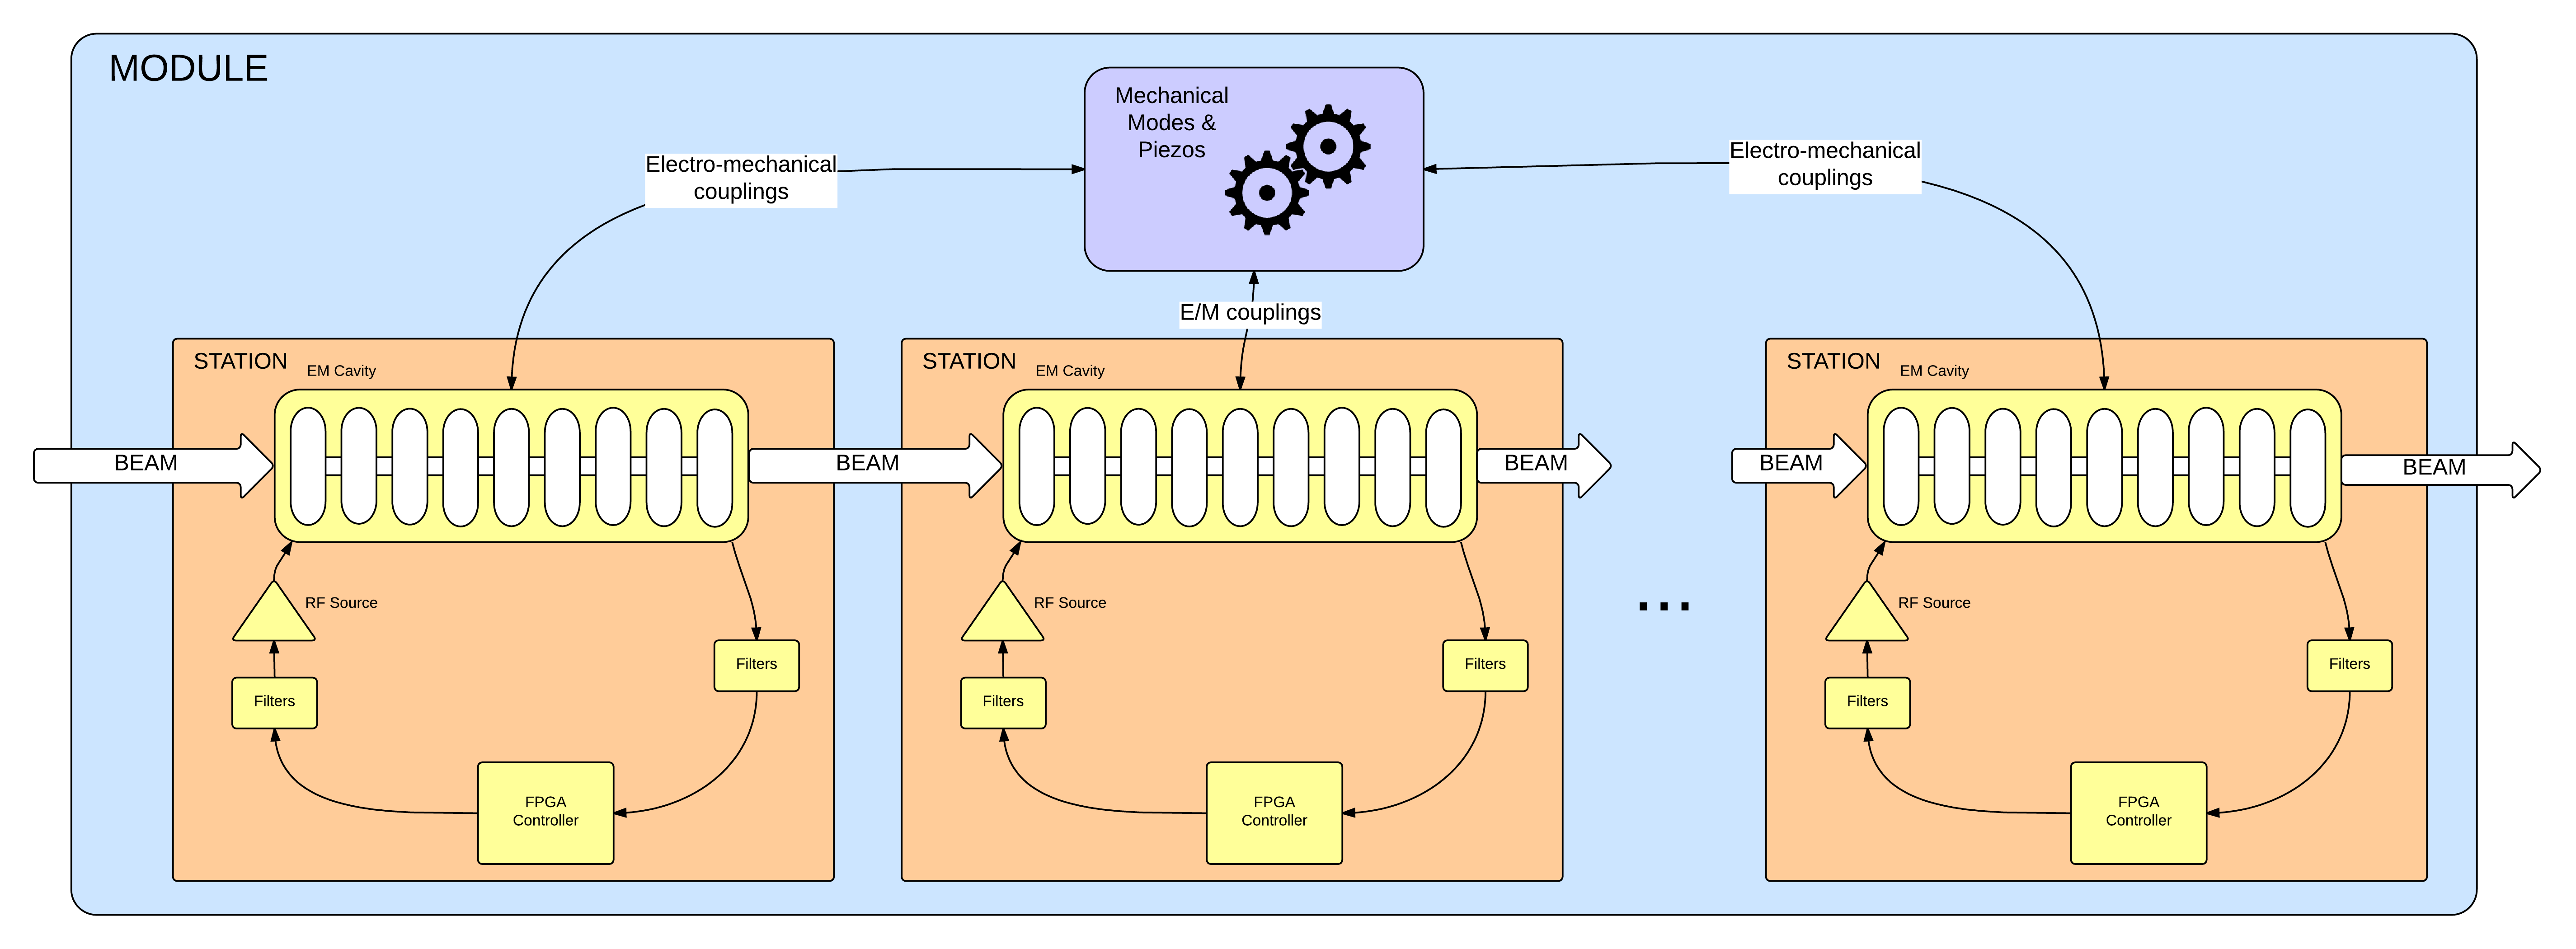
\includegraphics[scale=0.08]{../figures/Module_block_diagram.png}
\caption{Module block diagram.}
\label{fig:Module_block_diagram}
\end{figure}


\subsection{Mechanical model}

\section{Linac section}

\begin{figure}
\centering
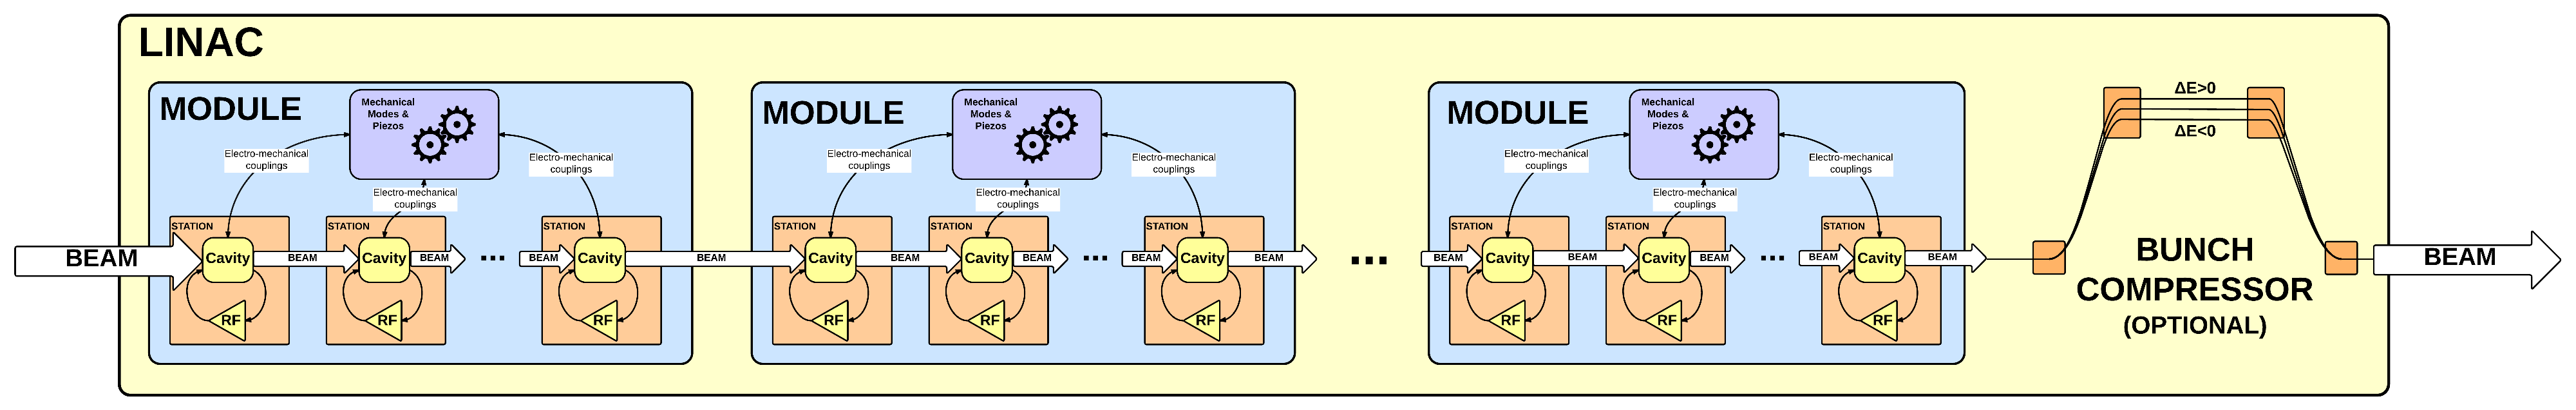
\includegraphics[scale=0.115]{../figures/Linac_block_diagram.png}
\caption{Linac block diagram.}
\label{fig:Linac_block_diagram}
\end{figure}

\subsection{Particle tracking model}



\subsection{Beam-based feedback model}


\begin{thebibliography}{19}   % Use for  1-9  references

\bibitem{ref:model-paper}
M. Mellado Munoz, L. Doolittle, P. Emma, G. Huang, A. Ratti, C. Serrano, J. M. Byrd, ``A Dynamic feedback model for high repetition rate LINAC-Driver FELs,''
IPAC'12, New Orleans, LA, May 2012.

\bibitem{ref:litrack} 
P. Emma, K. Bane, L. Freitag, ``LiTrack : A Fast longitudinal phase space tracking code with graphical user interface'', PAC'05,  Knoxville, TN, May 2005.

\bibitem{ref:superfish}
Poisson Superfish Software, \url{http://laacg.lanl.gov/laacg/services/download_sf.phtml}

\bibitem{ref:montgomery}
C. G. Montgomery, R. H. Dicke. E. M Purcell, ``Principles of Microwave Circuits'', MIT Radiation Lab Series V8, 1947.

\bibitem{ref:svea}
Slowly varying envelope approximation (SVEA), \url{http://en.wikipedia.org/wiki/Slowly_varying_envelope_approximation}.

\bibitem{ref:schilcher}
Vector Sum Control of Pulsed Accelerating Fields in Lorentz Force Detuned Superconducting Cavities, T. Schilcher, Hamburg 1998.


\end{thebibliography}

\end{document}